\newpage

\section{Project Execution}

\quad This section of the document is to describe the work done by each of the elements in the group. Each description will include each of the tasks completed by each group, the effort done for this work and the time spent doing this project.\\

For this work, we used a work methodology where, during the various meetings we held, we usually divided them into 3 parts. The first part consisted of analyzing the results of each of the team members, in case there were tasks to be done for that meeting. The second part of the meeting consists of analyzing what needs to be done in general for the next delivery, in that same time we visualized and aligned all the tasks to be done for the next presentation. Finally, the third and final part of the meeting consisted of dividing these tasks previously defined by each of the elements of the group.\\

We usually have at least 2 meetings in the space from one class to another, but there were situations where more than one meeting was necessary in that space of time, mainly due to doubts in the execution of the tasks, in these situations we normally gathered everyone by video call and resolved let's get to the problem. \\

\newpage

\subsection{Work Done By Dong Xuyong}

\quad For this project the tasks made by this member where:\\

\quad \textbullet Extract business objectives into features;\\

\quad \textbullet Model prediction with LSTM;\\

\quad \textbullet Reading the article “Understanding LSTM”;\\

\quad \textbullet Run all rminer ML models;\\

\quad \textbullet Parameter tuning for bud and stella;\\

\quad \textbullet Pipeline for all model types;\\

\quad \textbullet Analyze and run all models with all metrics for univariate variables, with different timelag combinations;\\

\quad \textbullet Growing and Rowling window;\\

\quad \textbullet Multivariate with VAR model and Arima with exogenous variables (precipitation and temperature);\\

\quad \textbullet Weakly Naive probability implementation and experience;\\

\quad \textbullet Fix the Weekly Naive template;\\

\quad \textbullet Implement the GW with neural networks with multivariate series and 2 outputs and model tuning in Python;\\

\quad \textbullet Analyze the optimization method.\\

This member of the group spent around 68 hours in this project;
\newpage

\subsection{Work Done By Pedro Silva}

\quad For this project the tasks made by this member where:\\

\quad \textbullet Extract business objectives into features;\\

\quad \textbullet Analysis of the exponential smoothing algorithm;\\

\quad \textbullet Research in GW and RW methods;\\

\quad \textbullet Search R tools;\\

\quad \textbullet Formulate the validation function;\\

\quad \textbullet See validation algorithms;\\

\quad \textbullet Think of a strategy on how to implement this same;\\

\quad \textbullet Implementation of the optimization method;\\

\quad \textbullet Interface implementation.\\


This member of the group spent around 65 hours in this project;
\newpage

\subsection{Work Done By Tiago Martins}

\quad For this project the tasks made by this member where:\\

\quad \textbullet Extract business objectives into features;\\

\quad \textbullet Analysis of Forecasting with Holt-Winters;\\

\quad \textbullet Research in GW and RW methods;\\

\quad \textbullet Final document development;\\

\quad \textbullet See validation algorithms;\\

\quad \textbullet Implementation of the optimization method;\\

\quad \textbullet Interface implementation.\\


This member of the group spent around 60 hours in this project;

\newpage

\subsection{The Work Methodology and Auto-Evaluation}

\quad For this work, we used a work methodology where, during the various meetings we held, we usually divided them into 3 parts. The first part consisted of analyzing the results of each of the team members, in case there were tasks to be done for that meeting. The second part of the meeting consists of analyzing what needs to be done in general for the next delivery, in that same time we visualized and aligned all the tasks to be done for the next presentation. Finally, the third and final part of the meeting consisted of dividing these tasks previously defined by each of the elements of the group.\\

We usually have at least 2 meetings in the space from one class to another, but there were situations where more than one meeting was necessary in that space of time, mainly due to doubts in the execution of the tasks, in these situations we normally gathered everyone by video call and resolved let's get to the problem. \\

For the Auto-Evaluation our group thinks this the grade that each element of the group deserves:
\\
\begin{figure}[H]
    \centering
    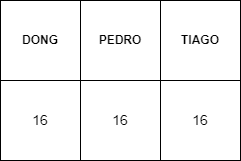
\includegraphics[width=0.4\textwidth]{assets/notas.png}
    \caption{Group Auto-Evaluation}
    \label{fig:notas}
    \end{figure}